\section{Observations}

\begin{itemize}
    \item Room temperature = 24.4 $^{\circ}$C = 297.55 K
    \item Length of glass plate (from the point of suspension) = 5.5 cm
    \item Wavelength of light used ($\lambda$)= 589.3 $\times$ 10$^{-9}$ m
\end{itemize}

\subsection*{Measurement of length of rod at room temperature}
Least count of vernier calipers = 0.01 cm
\begin{table}[H]
    \centering
    \begin{tabular}{|c|c|c|c|} \hline
        MSR (cm) & VSR (cm) & Total (cm) & $L_{RT}$ (cm) \\ \hline
        2 & 0.06 & 2.06 & \\
        2 & 0.07 & 2.07 & 2.063\\
        2 & 0.06 & 2.06 & \\
        \hline
        \end{tabular}    
        \caption{Measurement of the length of rod using a vernier caliper}
        \label{tab:2}
\end{table}

\subsection*{Measurement of fringe width ($\beta$)}
Least count of the travelling microscope = 0.01 mm
Data given in Table (\ref{tab:1}).
\begin{table*}
    \centering
\begin{ruledtabular}
    \begin{tabular}{|c|c|c|c|c|c|c|c|}
        \multicolumn{2}{|c|}{Temperature} & No. of  & Microscope  & Width of  & Avg. width  & Fringe width  & Wedge angle  \\ 
         in $^{\circ}$C & in K & Fringes & reading (mm) & 5 fringes (mm) & of 5 fringes (mm) & ($\beta$) (mm) & ($\theta$) in $10^{-3}$ rad \\
        \hline
        &            & 0  & 8.82 & - & & &  \\
        &            & 5  & 8.82 & 1.42 & & &  \\
        24.3 & 297.45 & 10 & 8.82 & 1.48 & 1.488 & 0.298 & 0.990 \\
        &            & 15 & 8.82 & 1.52 & & & \\
        &            & 20 & 8.82 & 1.53 & & & \\
        \hline
        &            & 0  & 8.77  & - & & &  \\
        &            & 5  & 10.04 & 1.27 & & &  \\
        37.7 & 310.85& 10 & 11.38 & 1.34 & 1.353 & 0.271 & 1.089 \\
        &            & 15 & 12.75 & 1.37 & & & \\
        &            & 20 & 14.18 & 1.43 & & & \\
        \hline
        &            & 0  & 8.99 & - & & &  \\
        &            & 5  & 10.26 & 1.27 & & &  \\
        48.0 & 321.15& 10 & 11.56 & 1.30 & 1.330 & 0.266 & 1.108 \\
        &            & 15 & 12.91 & 1.35 & & & \\
        &            & 20 & 14.31 & 1.40 & & & \\
        \hline
        &            & 0  & 9.09 & - & & &  \\
        &            & 5  & 10.24 & 1.15 & & &  \\
        58.4 & 331.55& 10 & 11.43 & 1.19 & 1.188 & 0.238 & 1.241 \\
        &            & 15 & 12.60 & 1.17 & & & \\
        &            & 20 & 13.84 & 1.24 & & & \\
        \hline
        &            & 0  & 8.94 & - & & &  \\
        &            & 5  & 10.02 & 1.08 & & &  \\
        75.0 & 348.15& 10 & 11.09 & 1.07 & 1.090 & 0.218 & 1.352 \\
        &            & 15 & 12.20 & 1.11 & & & \\
        &            & 20 & 13.30 & 1.10 & & & \\
        \hline
    \end{tabular}
    \end{ruledtabular} 
    \caption{Measurement of fringe width ($\beta$)}
    \label{tab:1}
\end{table*}

\section{Data Analysis and Calculations}

Using the data shown in Table (\ref{tab:1}), we make the following $\theta$ vs $T$ 
plot using least-square fitting.

\begin{figure}[H]
    \centering
    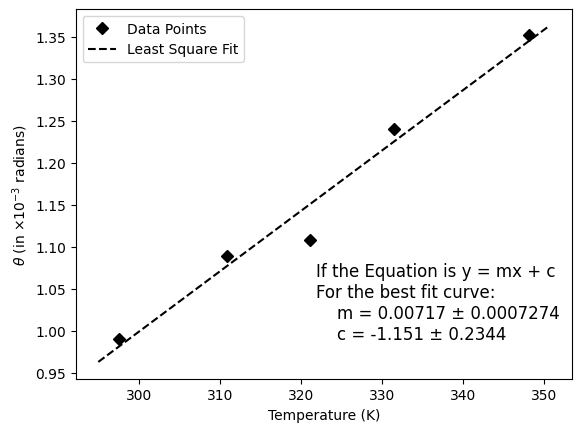
\includegraphics[width=1\columnwidth]{images/g1.png}
    \caption{$\theta$ vs $T$}
    \label{graph}
\end{figure}

Here slope of the $\theta$ vs $T$ plot comes out to be $m=0.007145 \times 10^{-3}$ K$^{-1}$. Using Eq. (8), we get,

\begin{align*}
    \alpha &= \frac{l}{L_{RT}} \times m\\
    &= \frac{5.5}{2.063} \times 0.00717 \times 10^{-3}\\
    &= 19.114 \times 10^{-3}\,\text{K}^{-1}
\end{align*}